\documentclass{llncs}\usepackage[]{graphicx}\usepackage[]{color}
%% maxwidth is the original width if it is less than linewidth
%% otherwise use linewidth (to make sure the graphics do not exceed the margin)
\makeatletter
\def\maxwidth{ %
  \ifdim\Gin@nat@width>\linewidth
    \linewidth
  \else
    \Gin@nat@width
  \fi
}
\makeatother

\definecolor{fgcolor}{rgb}{0.345, 0.345, 0.345}
\newcommand{\hlnum}[1]{\textcolor[rgb]{0.686,0.059,0.569}{#1}}%
\newcommand{\hlstr}[1]{\textcolor[rgb]{0.192,0.494,0.8}{#1}}%
\newcommand{\hlcom}[1]{\textcolor[rgb]{0.678,0.584,0.686}{\textit{#1}}}%
\newcommand{\hlopt}[1]{\textcolor[rgb]{0,0,0}{#1}}%
\newcommand{\hlstd}[1]{\textcolor[rgb]{0.345,0.345,0.345}{#1}}%
\newcommand{\hlkwa}[1]{\textcolor[rgb]{0.161,0.373,0.58}{\textbf{#1}}}%
\newcommand{\hlkwb}[1]{\textcolor[rgb]{0.69,0.353,0.396}{#1}}%
\newcommand{\hlkwc}[1]{\textcolor[rgb]{0.333,0.667,0.333}{#1}}%
\newcommand{\hlkwd}[1]{\textcolor[rgb]{0.737,0.353,0.396}{\textbf{#1}}}%

\usepackage{framed}
\makeatletter
\newenvironment{kframe}{%
 \def\at@end@of@kframe{}%
 \ifinner\ifhmode%
  \def\at@end@of@kframe{\end{minipage}}%
  \begin{minipage}{\columnwidth}%
 \fi\fi%
 \def\FrameCommand##1{\hskip\@totalleftmargin \hskip-\fboxsep
 \colorbox{shadecolor}{##1}\hskip-\fboxsep
     % There is no \\@totalrightmargin, so:
     \hskip-\linewidth \hskip-\@totalleftmargin \hskip\columnwidth}%
 \MakeFramed {\advance\hsize-\width
   \@totalleftmargin\z@ \linewidth\hsize
   \@setminipage}}%
 {\par\unskip\endMakeFramed%
 \at@end@of@kframe}
\makeatother

\definecolor{shadecolor}{rgb}{.97, .97, .97}
\definecolor{messagecolor}{rgb}{0, 0, 0}
\definecolor{warningcolor}{rgb}{1, 0, 1}
\definecolor{errorcolor}{rgb}{1, 0, 0}
\newenvironment{knitrout}{}{} % an empty environment to be redefined in TeX

\usepackage{alltt}
\usepackage{listings}
\usepackage{moreverb}
\usepackage{inconsolata}
\usepackage{amsmath}
\usepackage{stmaryrd}
\usepackage{bbm}
\pagestyle{plain}


\IfFileExists{upquote.sty}{\usepackage{upquote}}{}
\begin{document}

\title{Adaptive Rejection Sampling}
\author{
Thibault Doutre SID:26980469\\
Paul Cho SID:19642164\\
Zhenyuan Liu SID:26968476\\
Hao Lyu SID:26966632}
\institute{UC Berkeley}
\maketitle
\section{Intoduction}
By referring to the paper: "Rejection Sampling for Gibbs Sampling", we used the adaptive rejection sampling algorithm to simulate the samples for different log concave distributions. It mainly includes four different parts. The first part is Initialization, in this part we seek to find the initial bounds: x1 and xk, then we can generate the grid. Next we compute the upper hull and lower hull using the generated grid. After that we can do the sampling part by using the density $S_k$, calculated from the upper hull, and then update our grid after sampling some specific points. We also check the log concavity of our functions after each updating step. Finally we can repeat the sampling step to get the number of samples we want. We also tried as much as we can to vectorize and implement some tricks of generating a vector of samples but it is biased or inefficient compared to generating one point each time. We tested our results in four kinds of distributions and got the good results as shown in the tests part.\\
Zhenyuan Liu focused on developing the algorithm for initialization, adaptive rejection sampling, and updating as well as documentation. Thibault Doutre focused on finding an automated algorithm to reach x1 and xk in the initialization part, vectorizing the functions, testing and packaging. Hao Lyu focused on checking for log concavity and explored different algorithms for sampling efficiently. Paul Cho focused on vectorizing the functions, helped doing the R packaging, and implementing the help manual and documentation.\\
Github information: we worked on "doutib/ars".
\section{Initialization}
In this section our main purpose is to search for x1 and xk, which should lead to unbiased sampling and should never bring numerical issues. We set the default values for x1 and xk to be null, however, the author has the option to provide them. In this case, it would be faster to finish the sampling. The search for x1 and xk starts with a starting point x0 such that h(x0) is finite. If the domain is unbounded, it would be necessary to find a such x0, especially when the density function is shifted and the variance is small. If the domain of the distribution is bounded then we can use the bound to be our x0. The tricky part here is that when it comes to a distribution with very small variance, using constant step may either fail to find suitable x1 and xk or takes too long. So we used adaptive steps. We need to make our step smaller if it fails to find the reasonable x1,xk here.\\
For the upper hull, lower hull and envelop density, we just followed the definitions in the paper.
\section{Sampling and updating}
We used the Inverse CDF method to generate the sample from our envelop desity $S_k$ and do the two rejection tests to choose whether to keep the point or not. If a sampled point requires the rejection test, we will include it to the abscissae.
\section{Main function}
In our final version, we adopted the algorithm of sampling one point at a time. We also tried to first generate multiple points before performing the squeezing tests and the rejection tests. We expected this algorithm to be more efficient. However, this algorithn introduced more bias because it seemed as if samples were generated from less envelop densities because there was less updating steps. We also tried another algorithm. In this alorithm, we first generated m points, then kept all the points before the first point that failed the squeezing test. This particularly point had the chance to pass the rejection test. In this case it we didn't have any issues with bias, however, it was not faster as expected. We suspected that many of the mutiple points generated at once ended up being not sampled, thus increasing the samling time. Therefore we adopted the simple brute-force one-sample-one-test algorithm.
\section{Tests and results}
We used normal, gamma, beta and chi squared  distribution to test our samples and we campared the sample mean and variance with the true ones. We also plotted some histograms where the true distribution can be compared with the sample distribution. Finally we used the K-S tests to check whether the samples belongs to the true distribution. Large p-values indicates that we cannot reject the assumption that the samples are from the true distribution.
\begin{knitrout}
\definecolor{shadecolor}{rgb}{0.969, 0.969, 0.969}\color{fgcolor}\begin{kframe}


{\ttfamily\noindent\itshape\color{messagecolor}{\#\# Loading required package: testthat}}\begin{lstlisting}[basicstyle=\ttfamily,breaklines=true]
## main : 
## Computing test:  Beta(2,2).
\end{lstlisting}
\end{kframe}
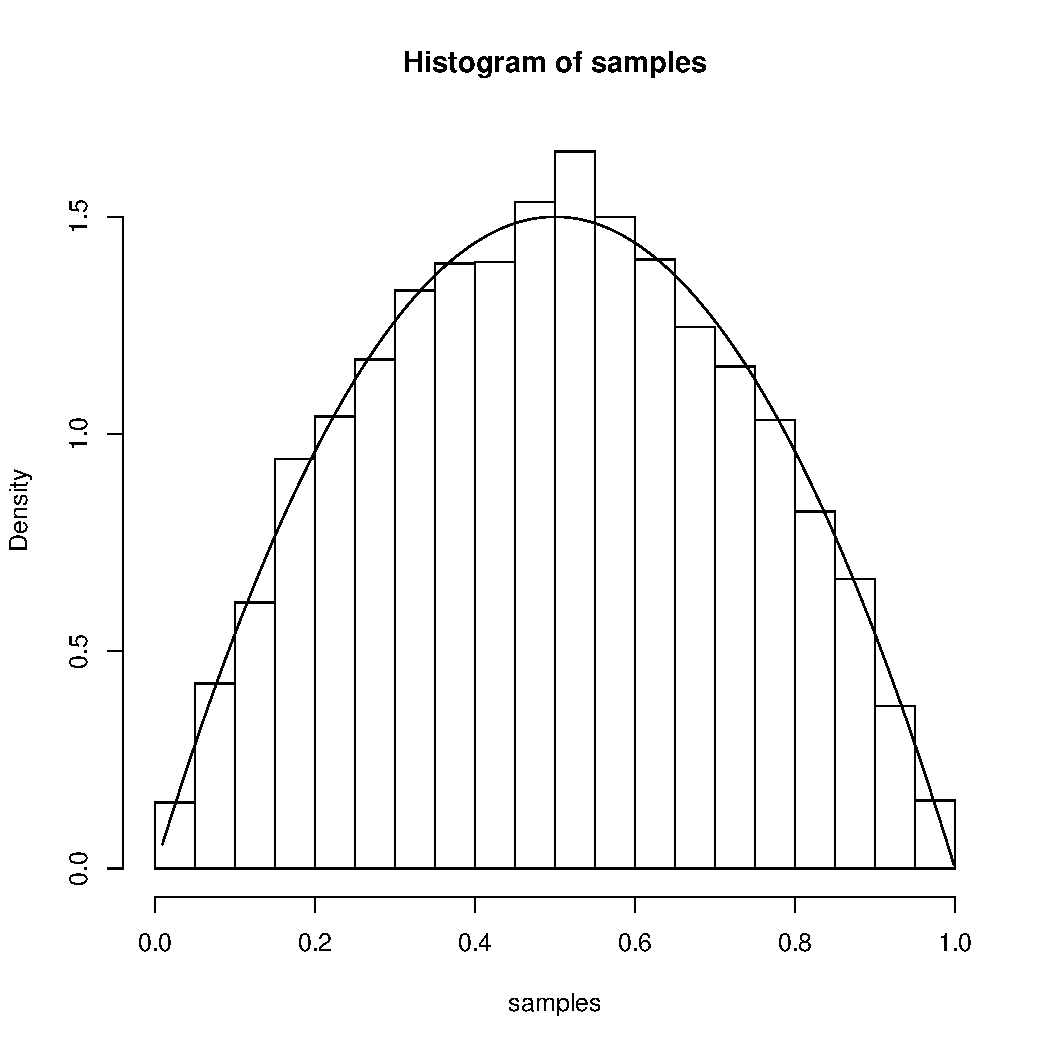
\includegraphics[width=\maxwidth]{figure/Rt-1} 
\begin{kframe}\begin{lstlisting}[basicstyle=\ttfamily,breaklines=true]
## 
## Result:
## D =  0.01011656 
## p-value =  0.2577146 
## ------------
## Computing test:  Beta(2,2).
\end{lstlisting}
\end{kframe}
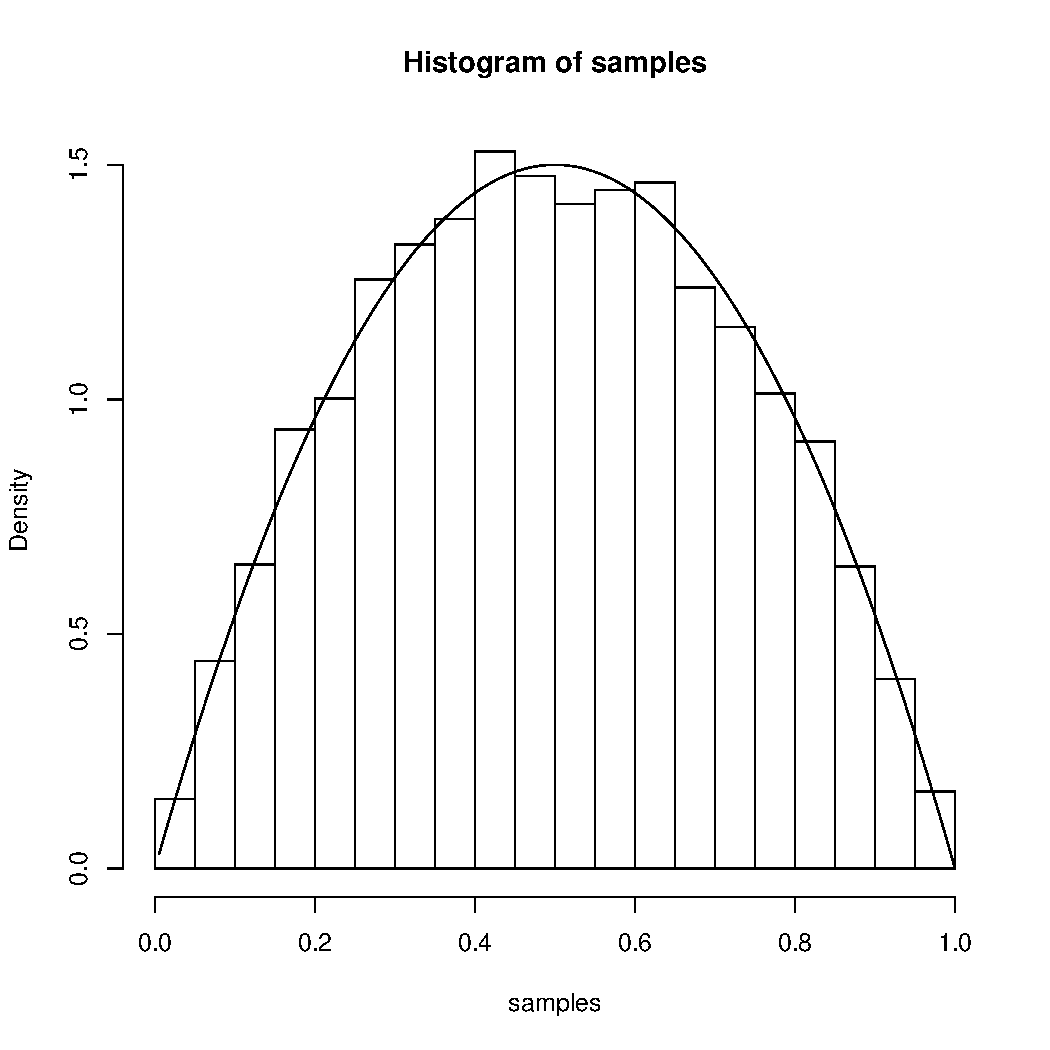
\includegraphics[width=\maxwidth]{figure/Rt-2} 
\begin{kframe}\begin{lstlisting}[basicstyle=\ttfamily,breaklines=true]
## 
## Result:
## D =  0.009945756 
## p-value =  0.2758934 
## ------------
## Computing test:  Beta(2,3).
\end{lstlisting}
\end{kframe}
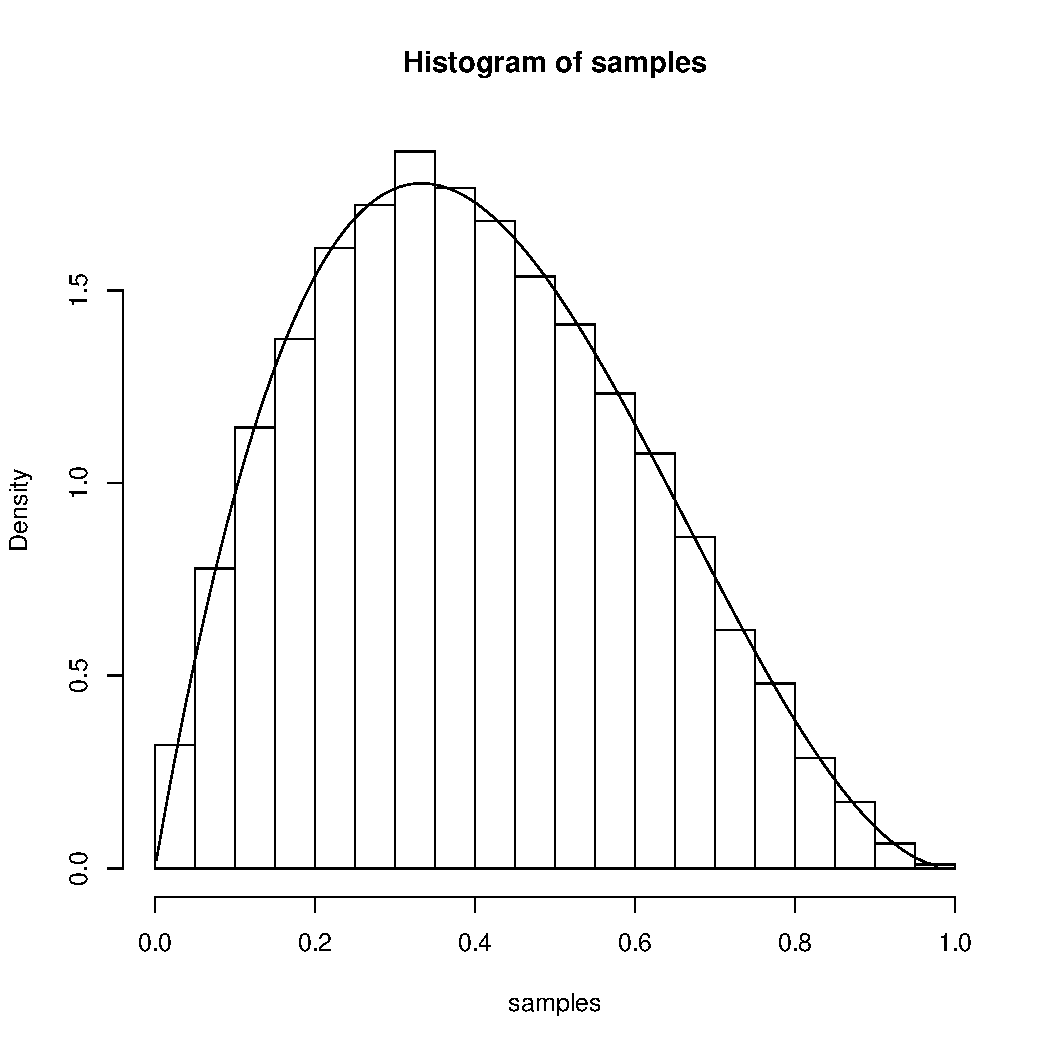
\includegraphics[width=\maxwidth]{figure/Rt-3} 
\begin{kframe}\begin{lstlisting}[basicstyle=\ttfamily,breaklines=true]
## 
## Result:
## D =  0.006446453 
## p-value =  0.8002559 
## ------------
## Computing test:  Beta(2,4).
\end{lstlisting}
\end{kframe}
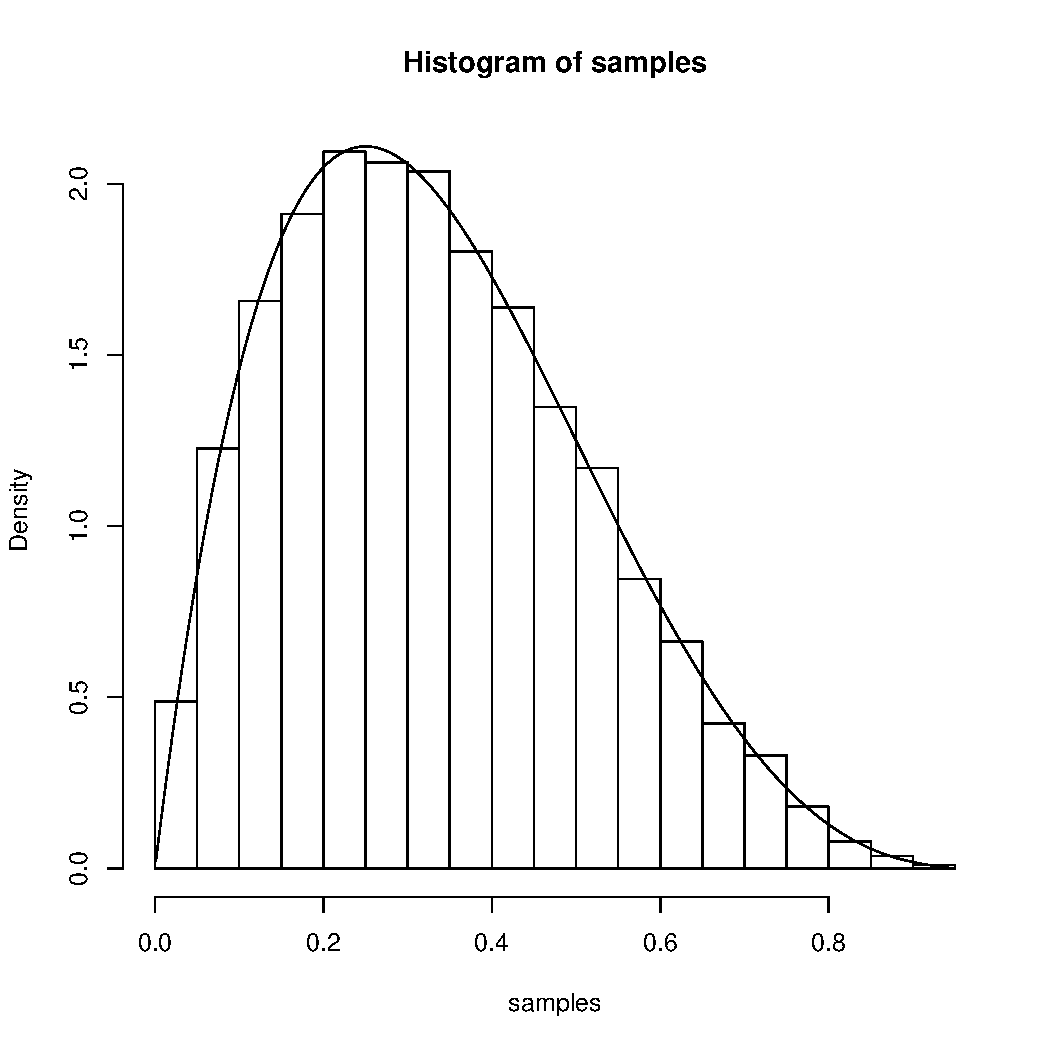
\includegraphics[width=\maxwidth]{figure/Rt-4} 
\begin{kframe}\begin{lstlisting}[basicstyle=\ttfamily,breaklines=true]
## 
## Result:
## D =  0.006620462 
## p-value =  0.7731233 
## ------------
## Computing test:  Beta(3,2)1
\end{lstlisting}
\end{kframe}
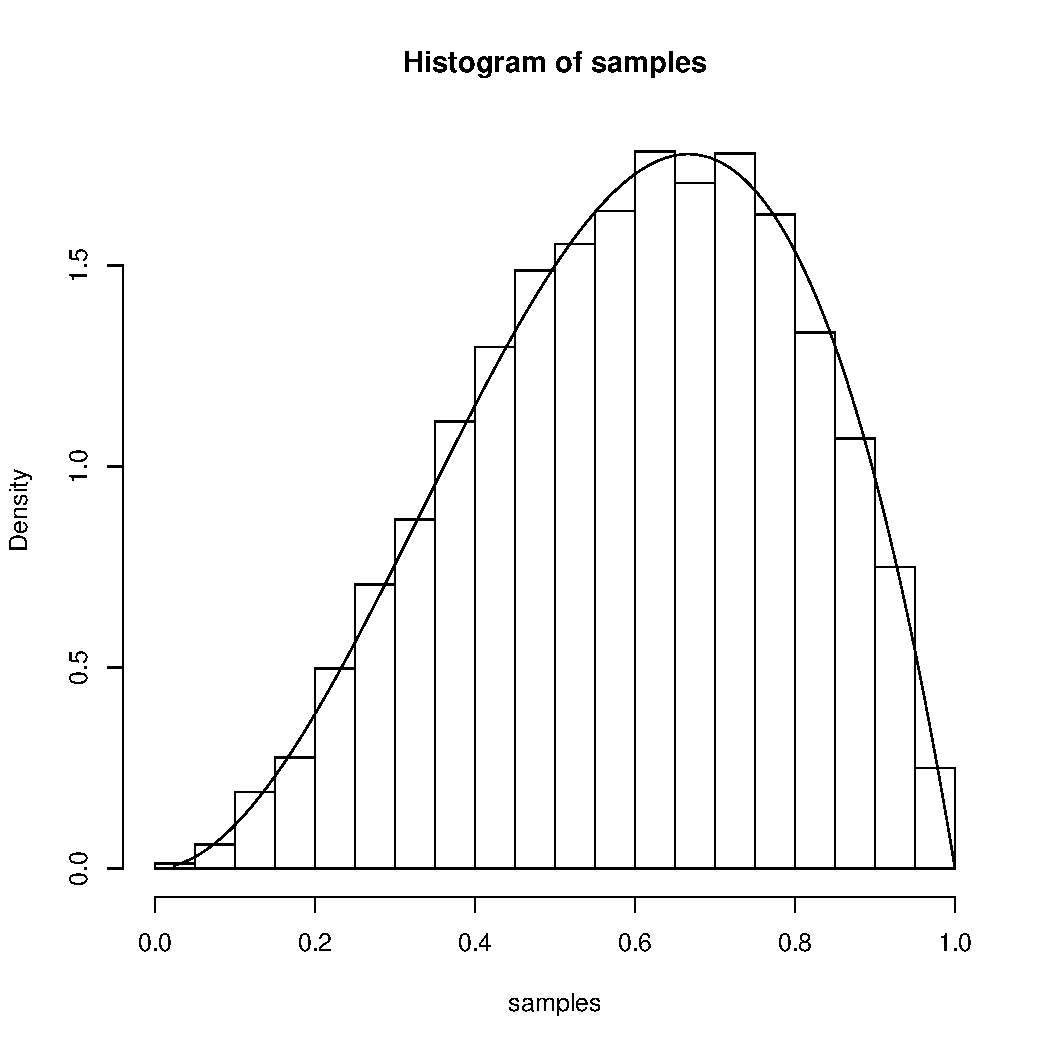
\includegraphics[width=\maxwidth]{figure/Rt-5} 
\begin{kframe}\begin{lstlisting}[basicstyle=\ttfamily,breaklines=true]
## 
## Result:
## D =  0.01508446 
## p-value =  0.02111708 
## ------------
## Computing test:  Beta(4,2).
\end{lstlisting}
\end{kframe}
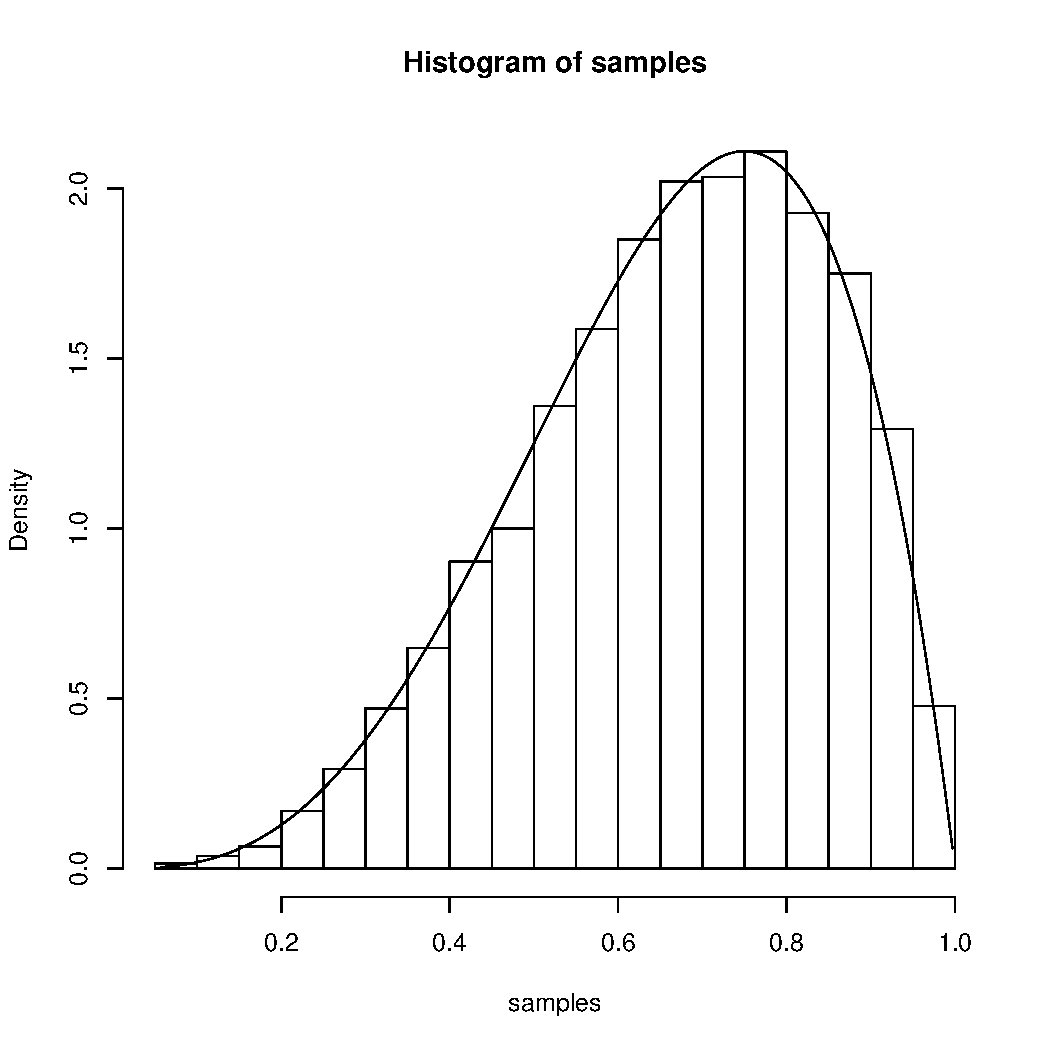
\includegraphics[width=\maxwidth]{figure/Rt-6} 
\begin{kframe}\begin{lstlisting}[basicstyle=\ttfamily,breaklines=true]
## 
## Result:
## D =  0.01356305 
## p-value =  0.05048935 
## ------------
## Computing test:  chisq(7).
\end{lstlisting}
\end{kframe}
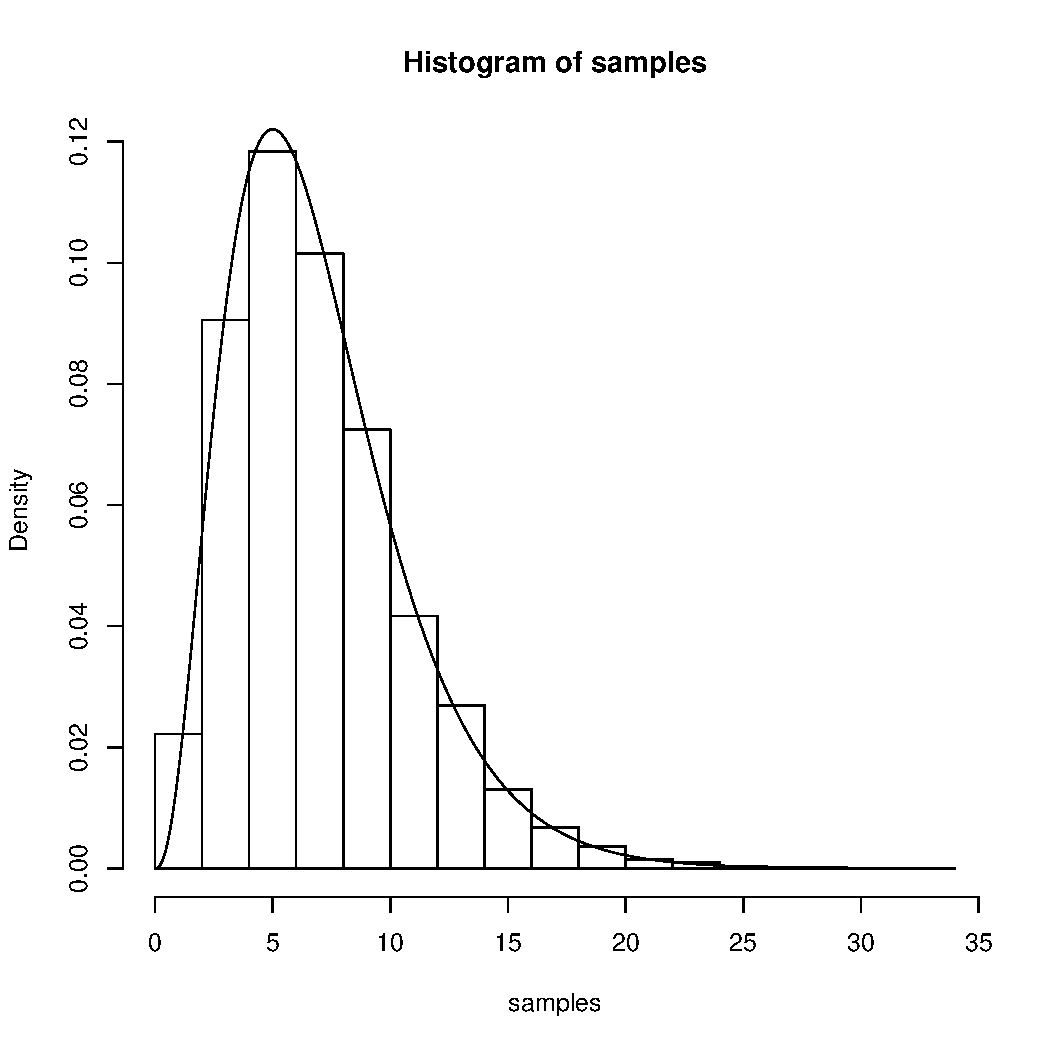
\includegraphics[width=\maxwidth]{figure/Rt-7} 
\begin{kframe}\begin{lstlisting}[basicstyle=\ttfamily,breaklines=true]
## 
## Result:
## D =  0.007385972 
## p-value =  0.6463855 
## ------------
## Computing test:  chisq(10).
\end{lstlisting}
\end{kframe}
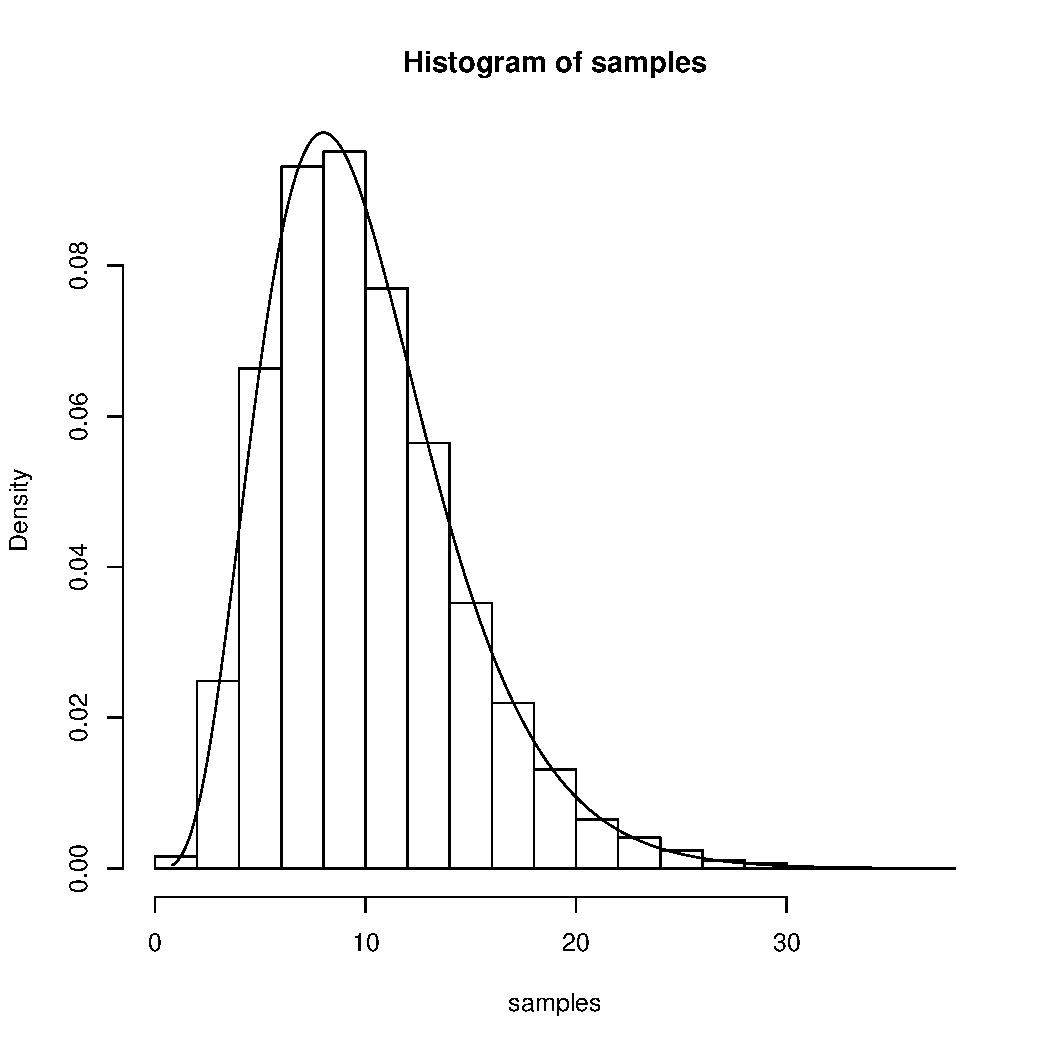
\includegraphics[width=\maxwidth]{figure/Rt-8} 
\begin{kframe}\begin{lstlisting}[basicstyle=\ttfamily,breaklines=true]
## 
## Result:
## D =  0.004952223 
## p-value =  0.9669189 
## ------------
## Computing test:  chisq(7)2
\end{lstlisting}
\end{kframe}
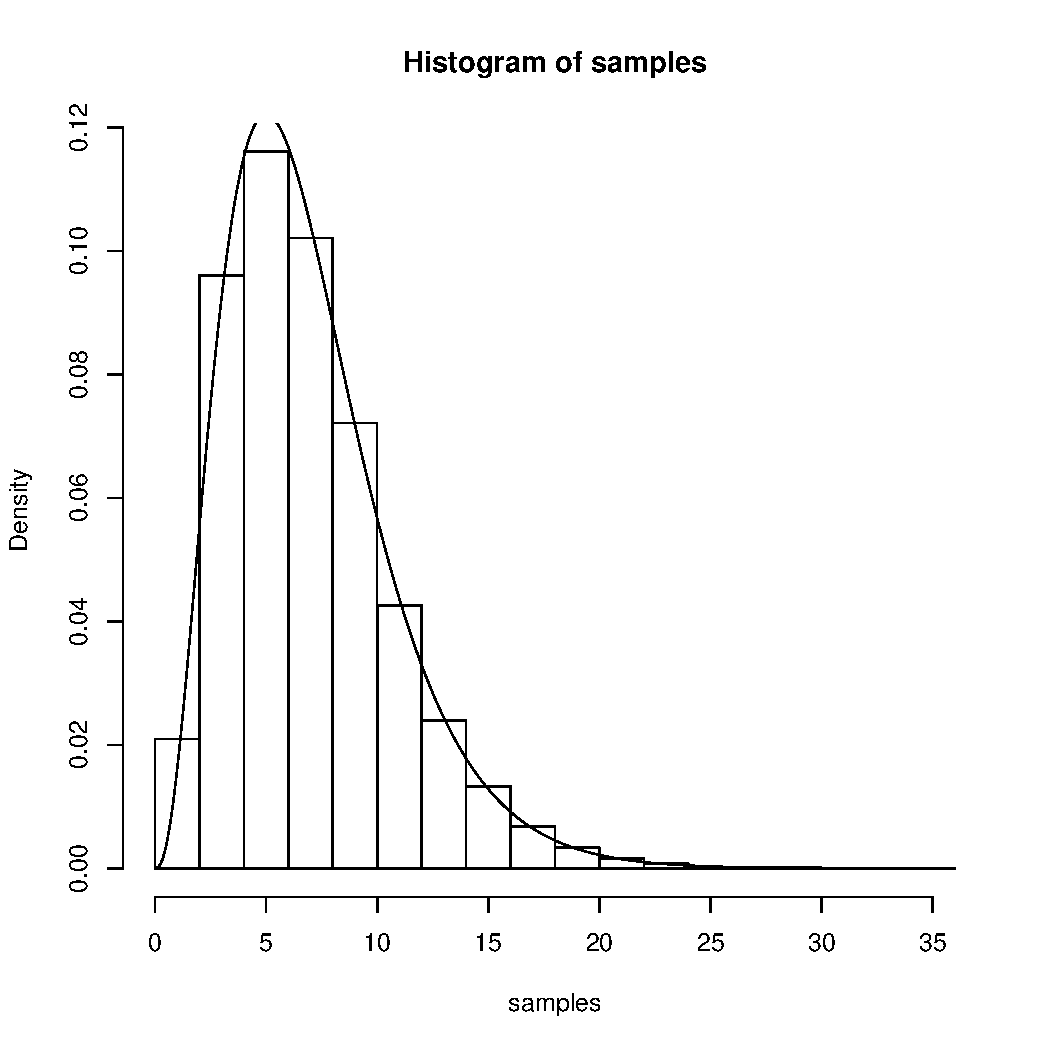
\includegraphics[width=\maxwidth]{figure/Rt-9} 
\begin{kframe}\begin{lstlisting}[basicstyle=\ttfamily,breaklines=true]
## 
## Result:
## D =  0.01469266 
## p-value =  0.02666674 
## ------------
## Computing test:  chisq(8).
\end{lstlisting}
\end{kframe}
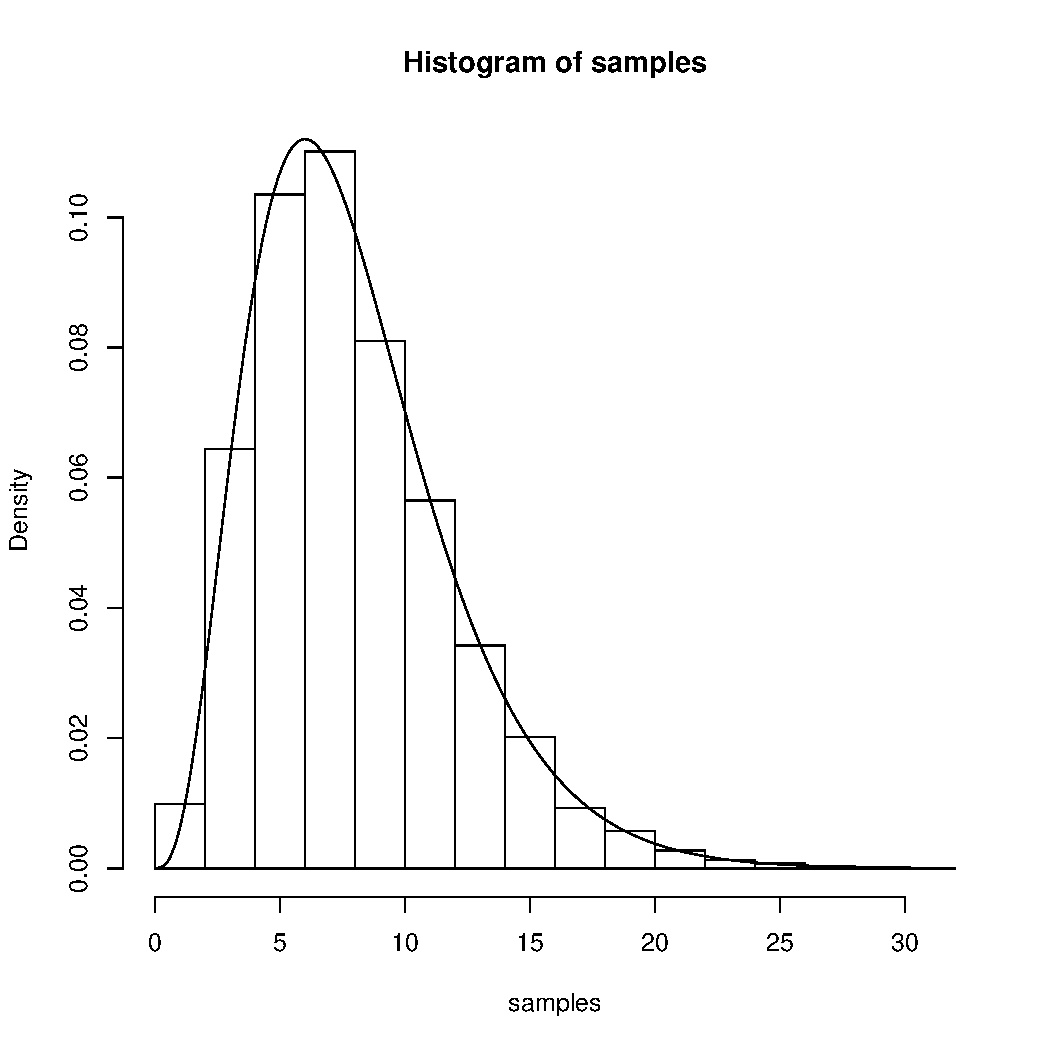
\includegraphics[width=\maxwidth]{figure/Rt-10} 
\begin{kframe}\begin{lstlisting}[basicstyle=\ttfamily,breaklines=true]
## 
## Result:
## D =  0.01173555 
## p-value =  0.1272534 
## ------------
## Computing test:  chisq(9).
\end{lstlisting}
\end{kframe}
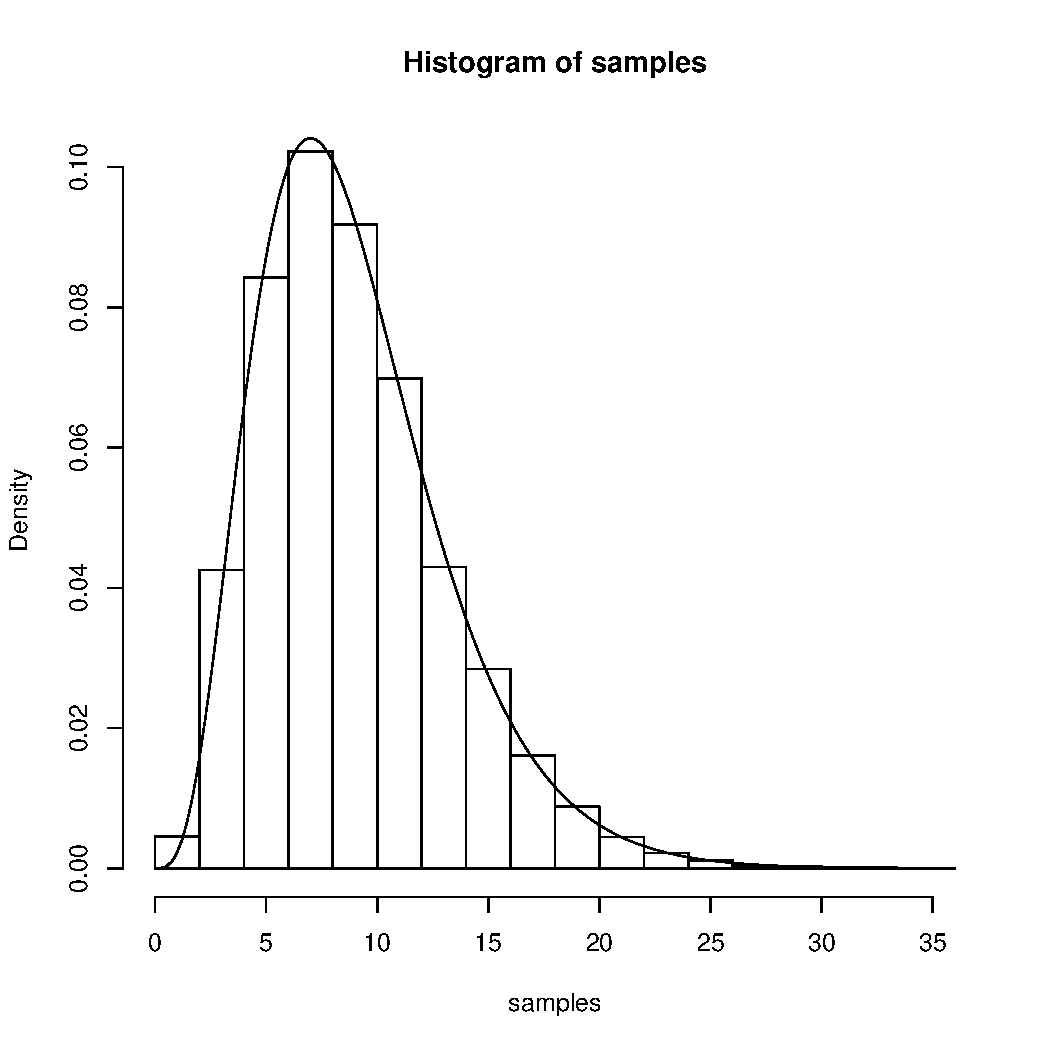
\includegraphics[width=\maxwidth]{figure/Rt-11} 
\begin{kframe}\begin{lstlisting}[basicstyle=\ttfamily,breaklines=true]
## 
## Result:
## D =  0.005738556 
## p-value =  0.8968943 
## ------------
## Computing test:  Gamma(shape=4).
\end{lstlisting}
\end{kframe}
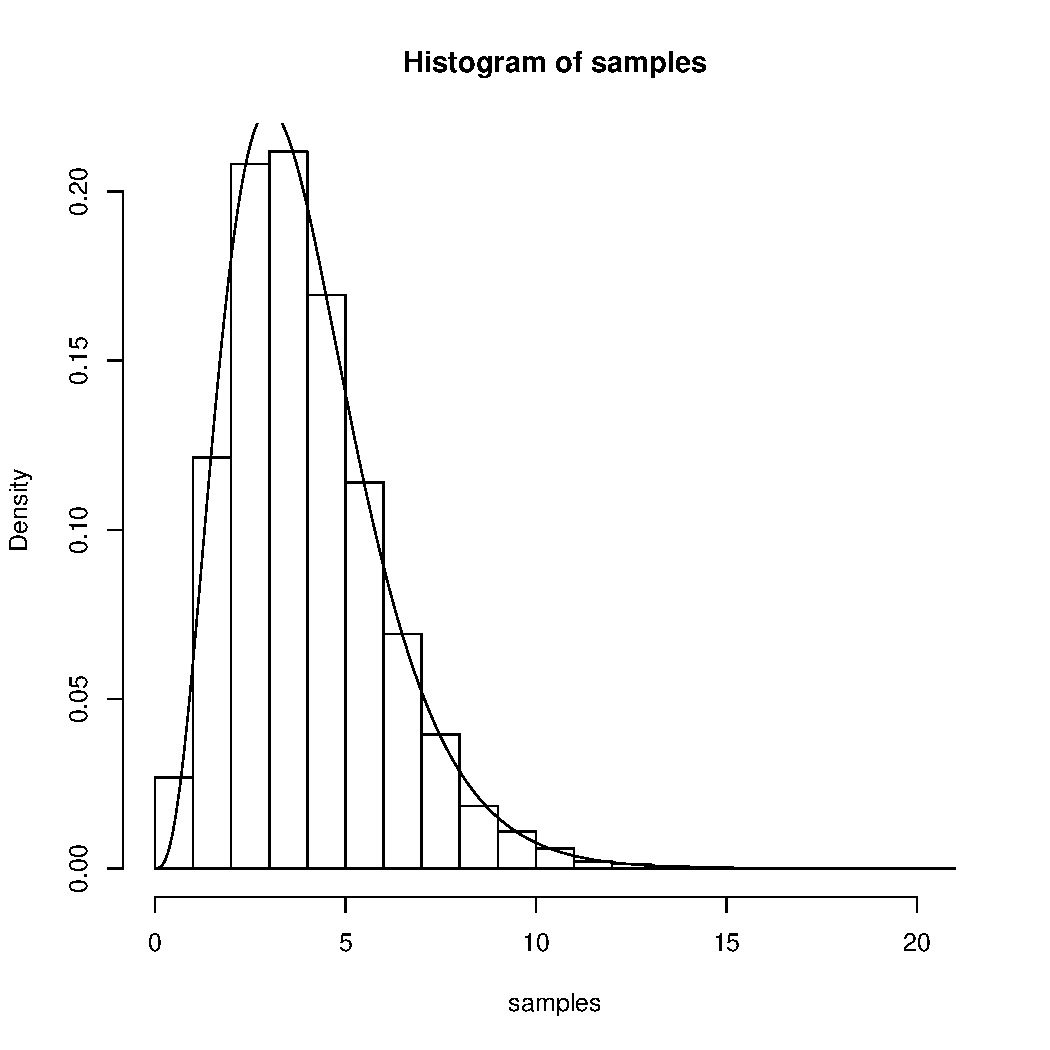
\includegraphics[width=\maxwidth]{figure/Rt-12} 
\begin{kframe}\begin{lstlisting}[basicstyle=\ttfamily,breaklines=true]
## 
## Result:
## D =  0.008216175 
## p-value =  0.5094048 
## ------------
## Computing test:  Gamma(shape=5).
\end{lstlisting}
\end{kframe}
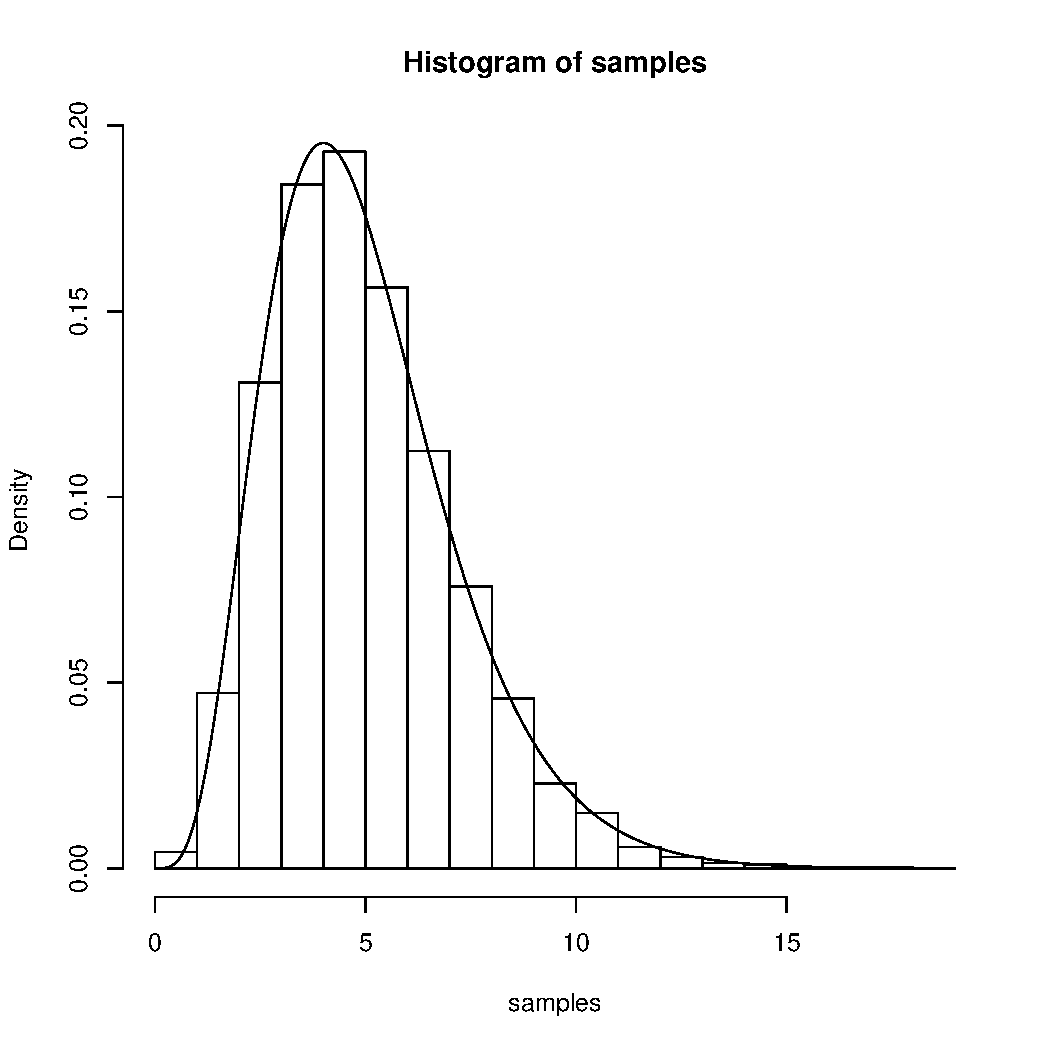
\includegraphics[width=\maxwidth]{figure/Rt-13} 
\begin{kframe}\begin{lstlisting}[basicstyle=\ttfamily,breaklines=true]
## 
## Result:
## D =  0.007527043 
## p-value =  0.6226162 
## ------------
## Computing test:  Gamma(shape=6).
\end{lstlisting}
\end{kframe}
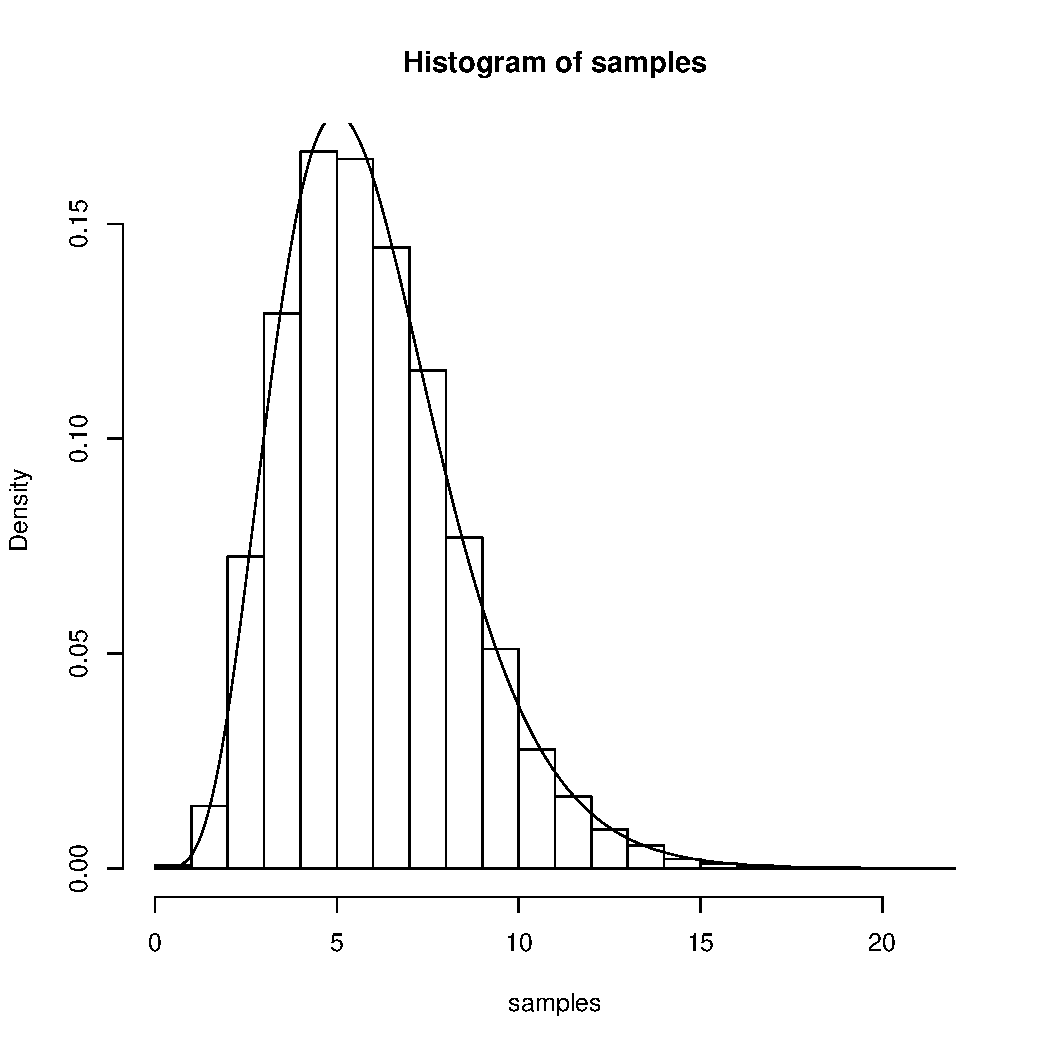
\includegraphics[width=\maxwidth]{figure/Rt-14} 
\begin{kframe}\begin{lstlisting}[basicstyle=\ttfamily,breaklines=true]
## 
## Result:
## D =  0.007875892 
## p-value =  0.5644607 
## ------------
## Computing test:  Gamma(shape=7)3
\end{lstlisting}
\end{kframe}
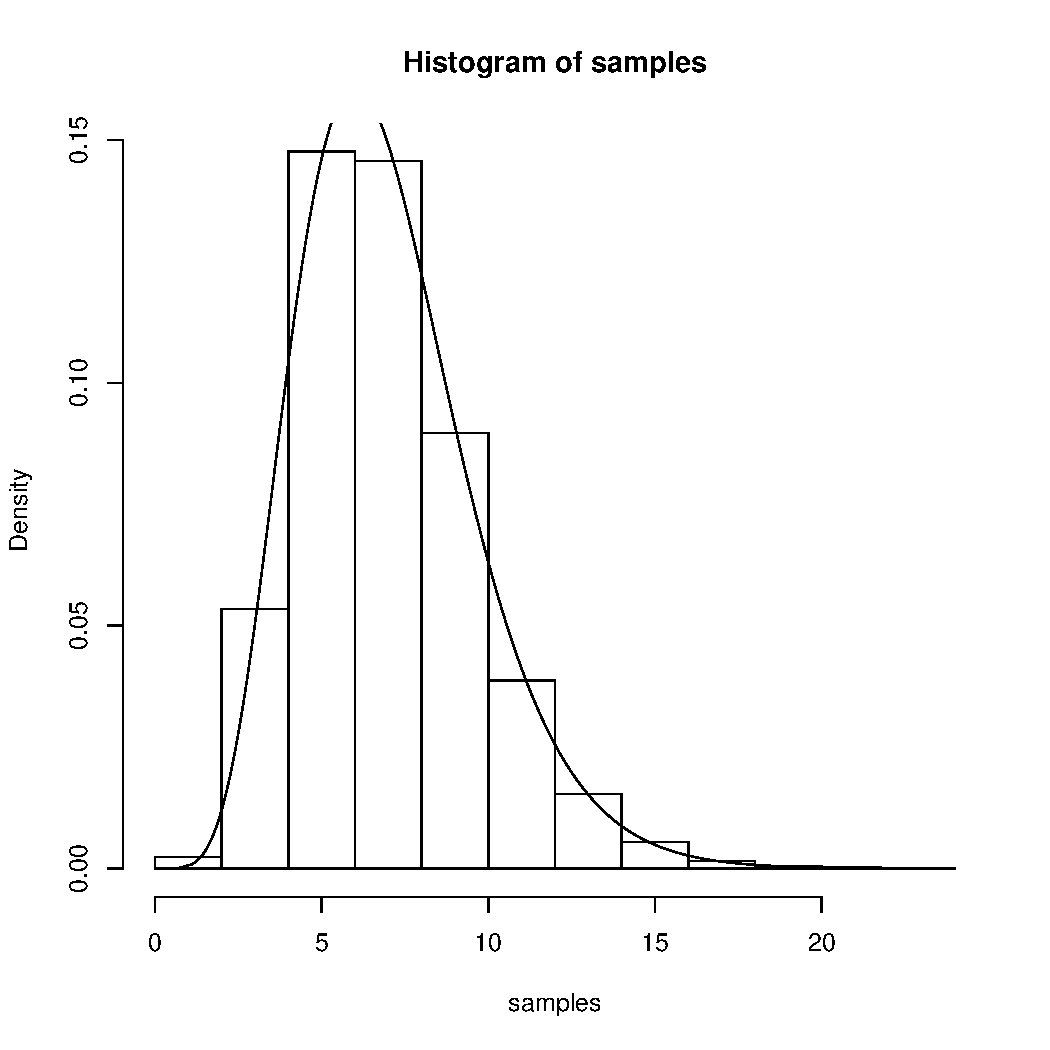
\includegraphics[width=\maxwidth]{figure/Rt-15} 
\begin{kframe}\begin{lstlisting}[basicstyle=\ttfamily,breaklines=true]
## 
## Result:
## D =  0.01646203 
## p-value =  0.008854596 
## ------------
## Computing test:  Gamma(shape=8).
\end{lstlisting}
\end{kframe}
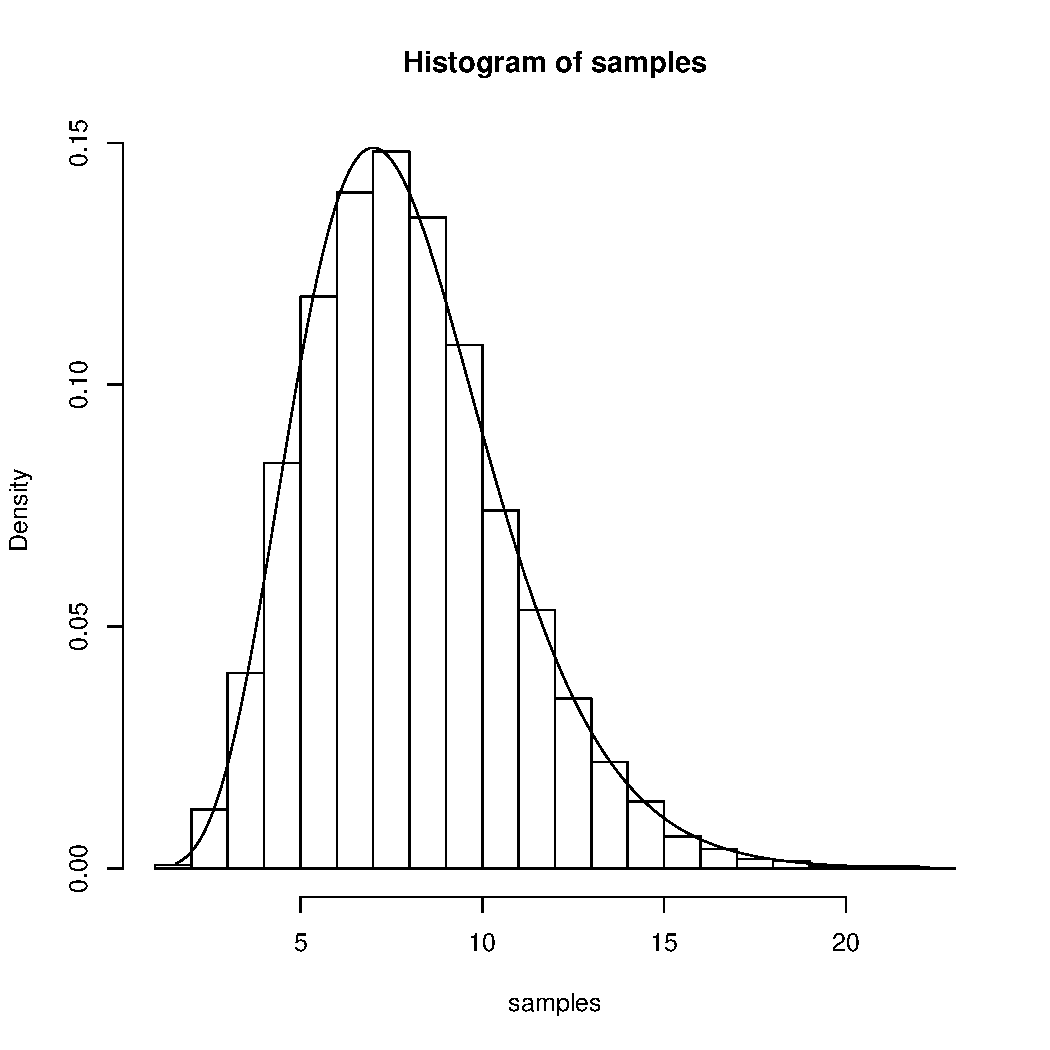
\includegraphics[width=\maxwidth]{figure/Rt-16} 
\begin{kframe}\begin{lstlisting}[basicstyle=\ttfamily,breaklines=true]
## 
## Result:
## D =  0.009540994 
## p-value =  0.3224919 
## ------------
## Computing test:  N(9737.67,0.1).
\end{lstlisting}
\begin{lstlisting}[basicstyle=\ttfamily,breaklines=true]
## 
## Result:
## D =  0.01258734 
## p-value =  0.08409988 
## ------------
## Computing test:  N(9737.67,0.01)
\end{lstlisting}


{\ttfamily\noindent\color{warningcolor}{\#\# Warning in ks.test(samples, true\_cdf, ...): ties should not be present for the Kolmogorov-Smirnov test}}\end{kframe}
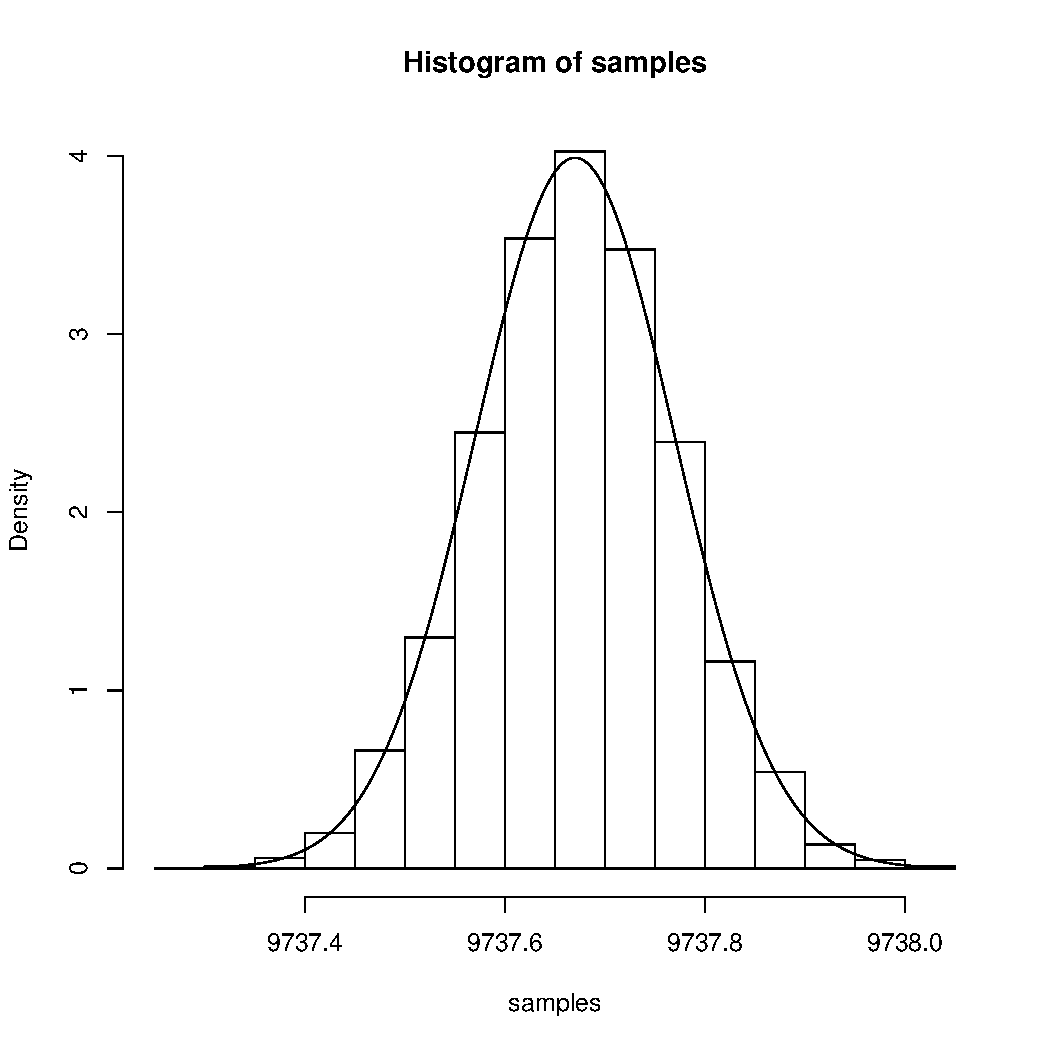
\includegraphics[width=\maxwidth]{figure/Rt-17} 
\begin{kframe}\begin{lstlisting}[basicstyle=\ttfamily,breaklines=true]
## .
\end{lstlisting}
\end{kframe}
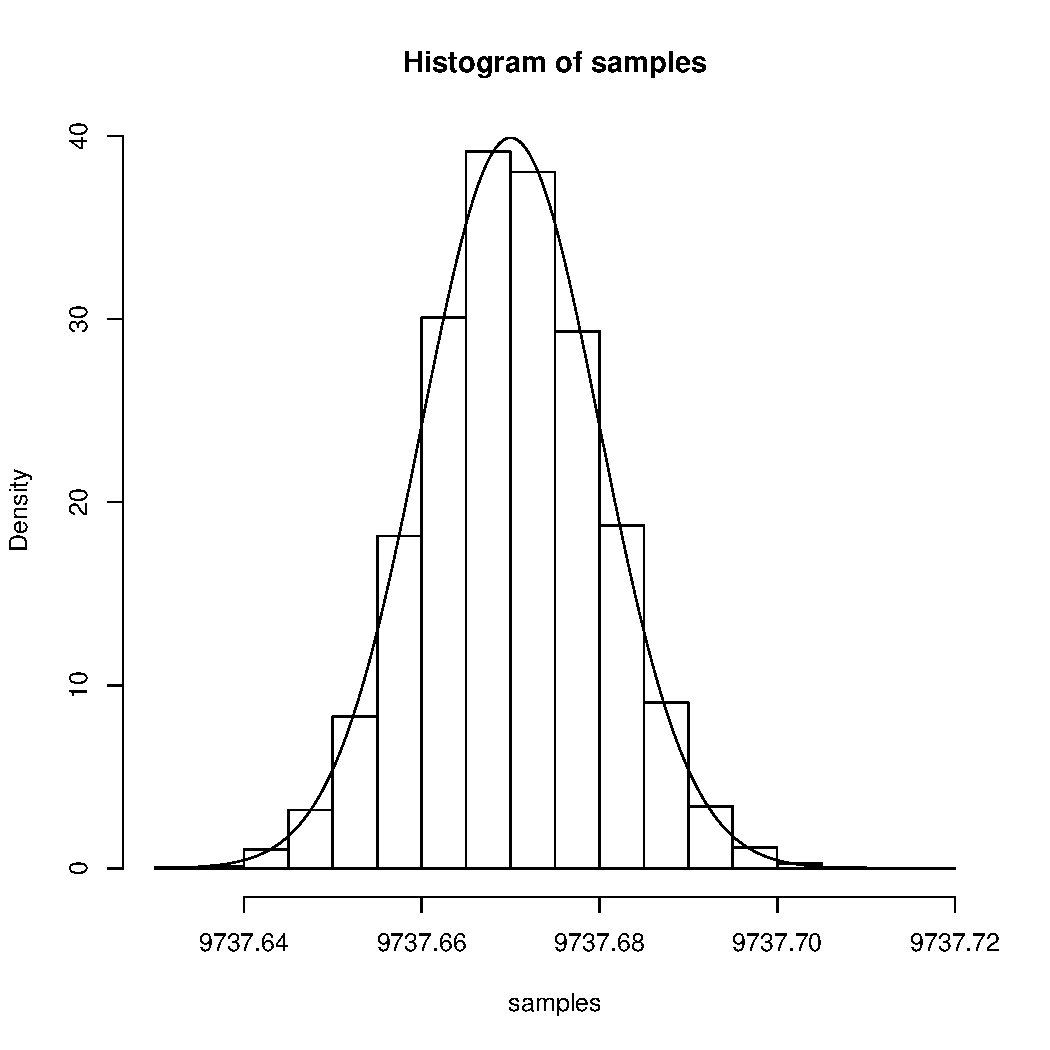
\includegraphics[width=\maxwidth]{figure/Rt-18} 
\begin{kframe}\begin{lstlisting}[basicstyle=\ttfamily,breaklines=true]
## 
## Result:
## D =  0.007833838 
## p-value =  0.5713985 
## ------------
## Computing test:  N(2,0.1).
\end{lstlisting}
\end{kframe}
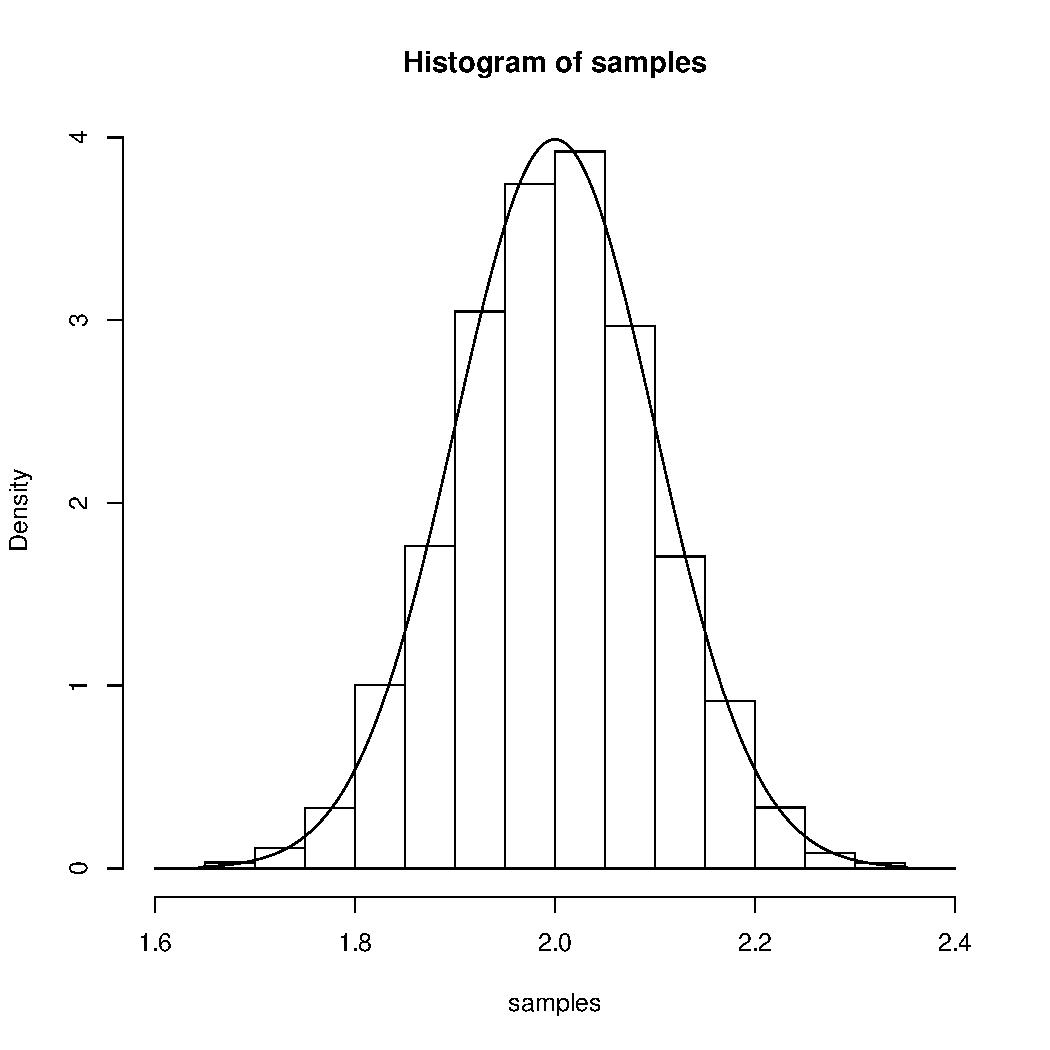
\includegraphics[width=\maxwidth]{figure/Rt-19} 
\begin{kframe}\begin{lstlisting}[basicstyle=\ttfamily,breaklines=true]
## 
## Result:
## D =  0.008718832 
## p-value =  0.4326999 
## ------------
## Computing test:  N(9737.67,0.1).
\end{lstlisting}
\end{kframe}
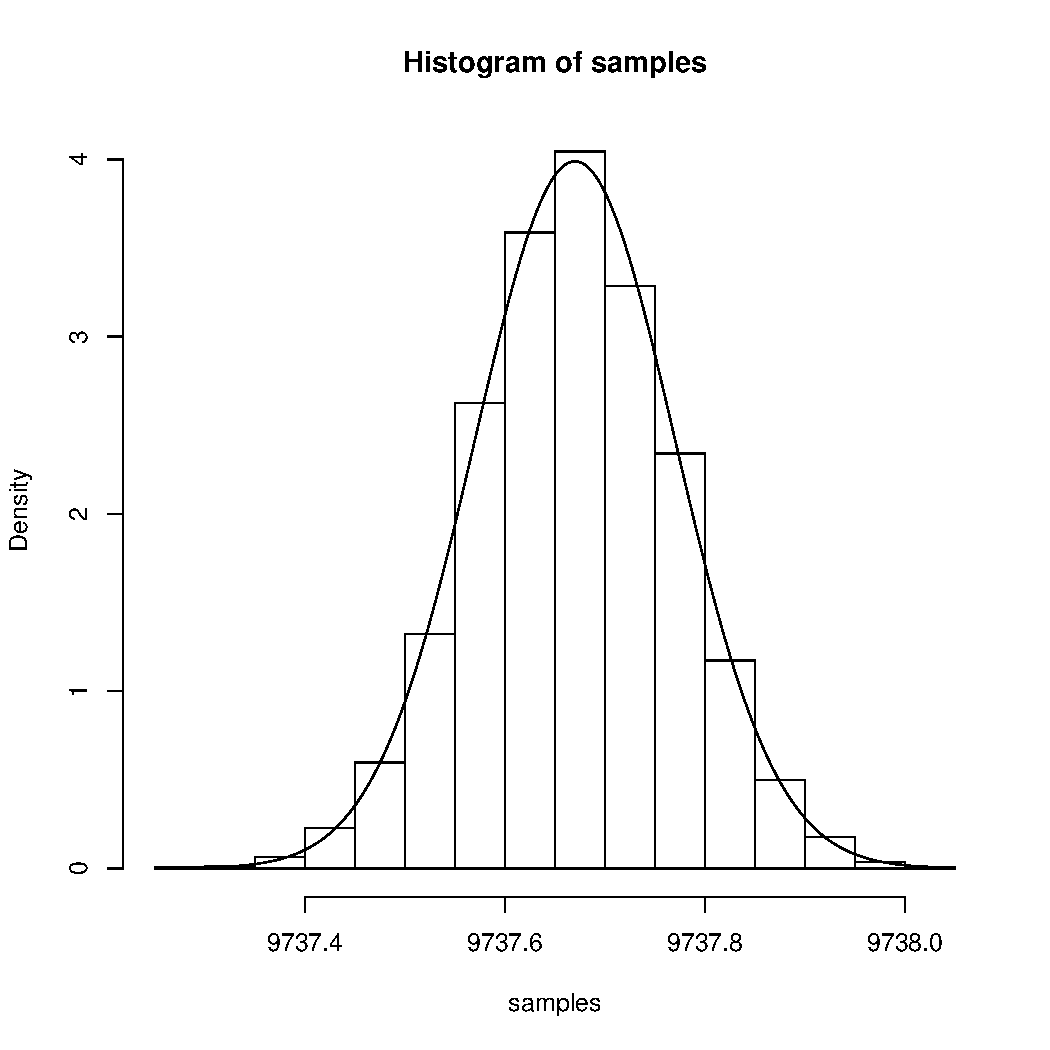
\includegraphics[width=\maxwidth]{figure/Rt-20} 
\begin{kframe}\begin{lstlisting}[basicstyle=\ttfamily,breaklines=true]
## 
## Result:
## D =  0.007731778 
## p-value =  0.5883313 
## ------------
## Computing test:  N(9737.67,1).
\end{lstlisting}
\begin{lstlisting}[basicstyle=\ttfamily,breaklines=true]
## 
## Result:
## D =  0.007590487 
## p-value =  0.6119563 
## ------------
## Computing test:  N(-9737.67,0.01)
\end{lstlisting}


{\ttfamily\noindent\color{warningcolor}{\#\# Warning in ks.test(samples, true\_cdf, ...): ties should not be present for the Kolmogorov-Smirnov test}}\end{kframe}
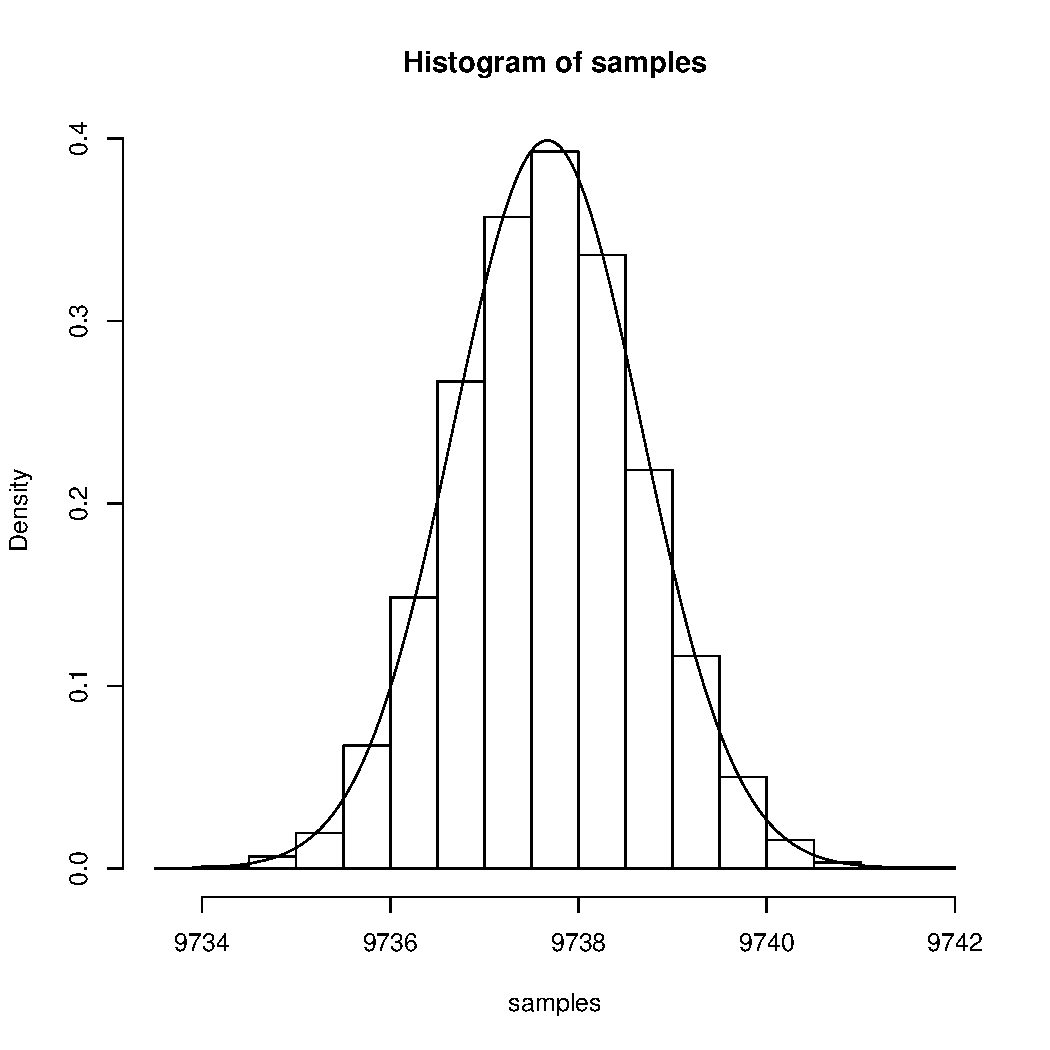
\includegraphics[width=\maxwidth]{figure/Rt-21} 
\begin{kframe}\begin{lstlisting}[basicstyle=\ttfamily,breaklines=true]
## .
\end{lstlisting}
\end{kframe}
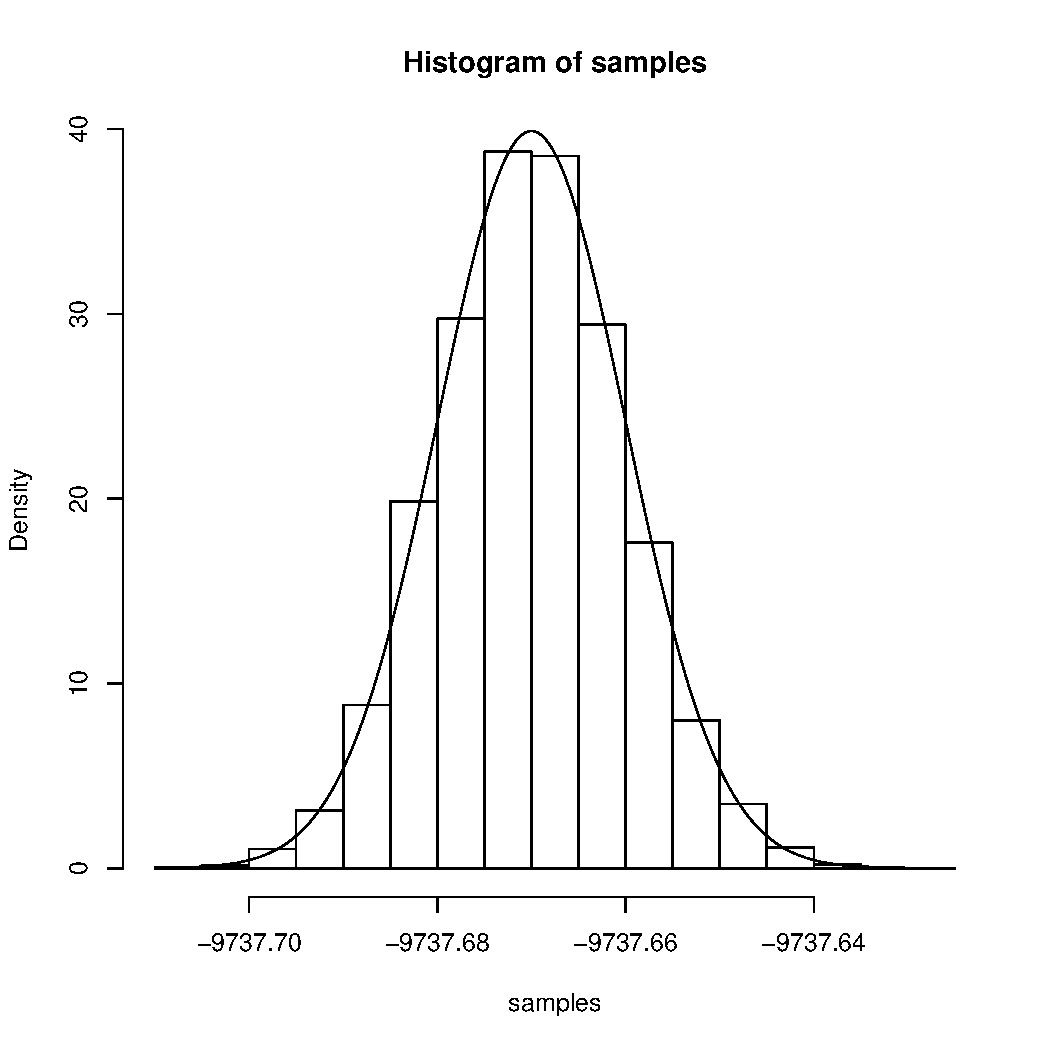
\includegraphics[width=\maxwidth]{figure/Rt-22} 
\begin{kframe}\begin{lstlisting}[basicstyle=\ttfamily,breaklines=true]
## 
## Result:
## D =  0.01189722 
## p-value =  0.1178981 
## ------------
## Computing test:  N(-9737.67,0.1).
\end{lstlisting}
\begin{lstlisting}[basicstyle=\ttfamily,breaklines=true]
## 
## Result:
## D =  0.004825747 
## p-value =  0.9740105 
## ------------
## Computing test:  N(-9737.67,0.1)
\end{lstlisting}


{\ttfamily\noindent\color{warningcolor}{\#\# Warning in ks.test(samples, true\_cdf, ...): ties should not be present for the Kolmogorov-Smirnov test}}\end{kframe}
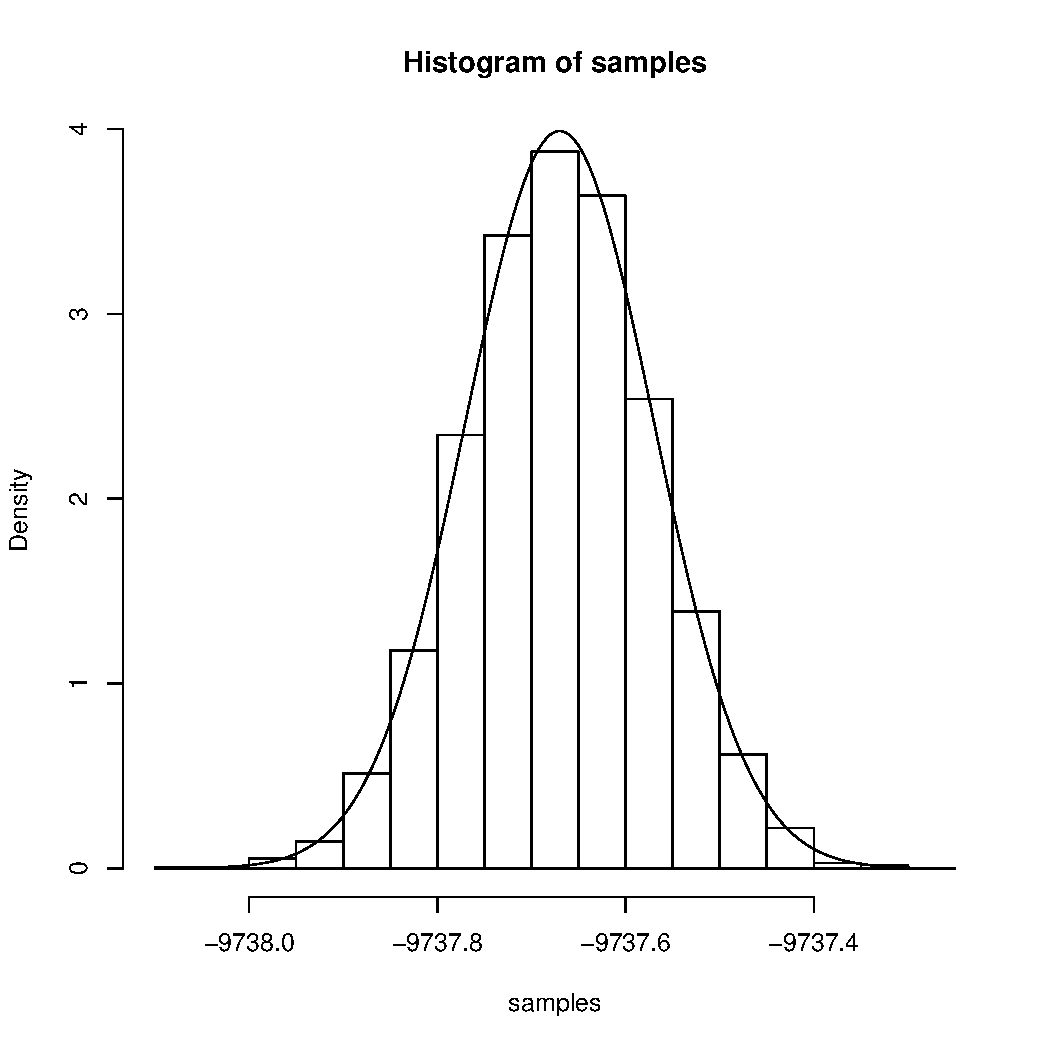
\includegraphics[width=\maxwidth]{figure/Rt-23} 
\begin{kframe}\begin{lstlisting}[basicstyle=\ttfamily,breaklines=true]
## .
\end{lstlisting}
\end{kframe}
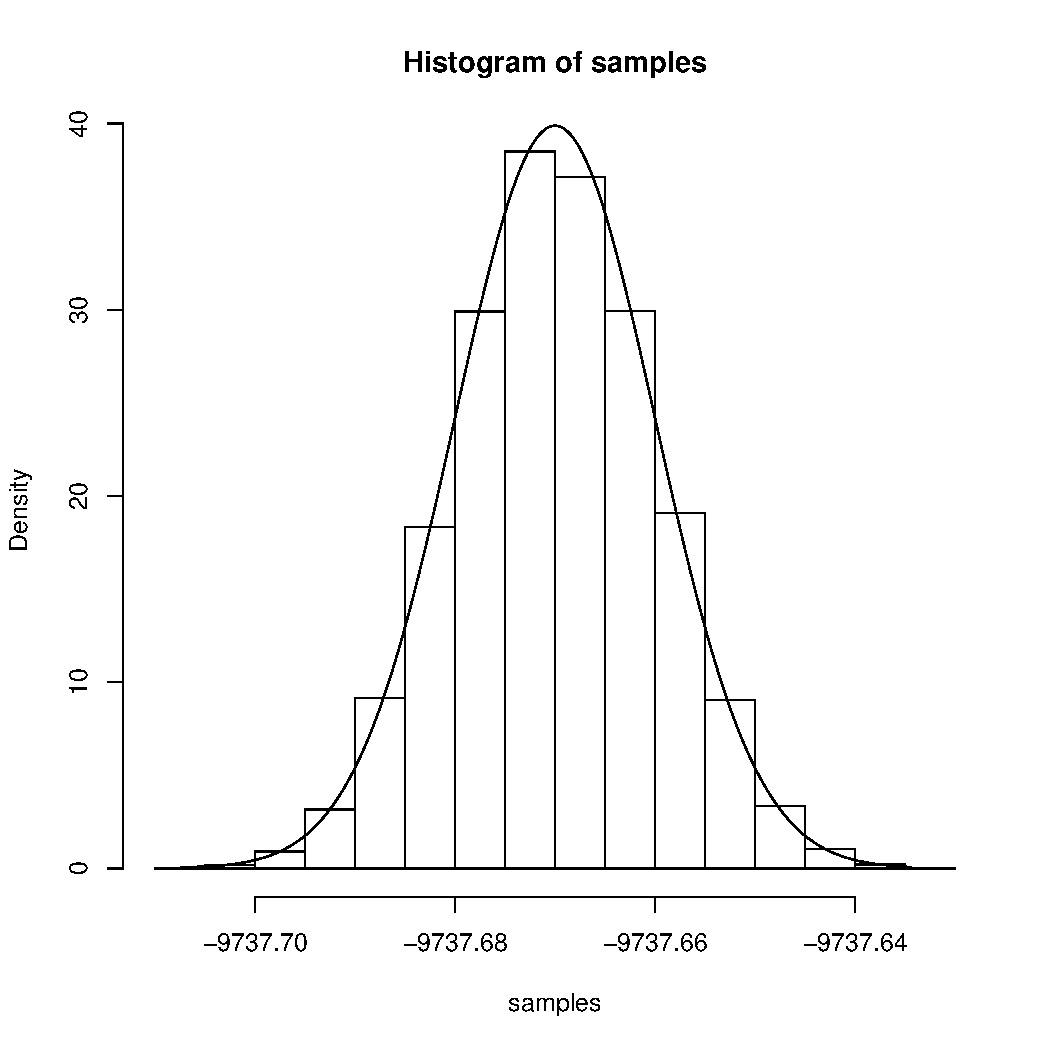
\includegraphics[width=\maxwidth]{figure/Rt-24} 
\begin{kframe}\begin{lstlisting}[basicstyle=\ttfamily,breaklines=true]
## 
## Result:
## D =  0.007822811 
## p-value =  0.5732215 
## ------------
## 1. Failure: Beta(3,2) --------------------------------------
## ks_test$p.value >= pvalue isn't true
## 
## 2. Failure: chisq(7) ---------------------------------------
## ks_test$p.value >= pvalue isn't true
## 
## 3. Failure: Gamma(shape=7) ---------------------------------
## ks_test$p.value >= pvalue isn't true
\end{lstlisting}
\end{kframe}
\end{knitrout}
\section{Appendix: Description of Each Auxiliary Function}

\subsection{search(h,domain)}
It can search for a x0 such that h(x0) is finite and the gradient of h at x0 is attained. This is particular useful when the domain is unbounded, the mode is far away from 0 (yet unknown) and the variance is very small, i.e. the density function is very narrow. In such cases, it's even difficult to make a guess for an initial value to find x1 and xk.\\
\textbf{Usage}:\\
\begin{verbatim}
search(h,domain,x_start,max_x,min_step,relax_factor)
\end{verbatim}
\textbf{Arguments}:\\
\begin{verbatim}
h: the log of the density function
domain: the domain of the density function
x_start: the starting x value for the search
max_x: the maximum search limit for x, if the mode is shifted beyond this limit, the user should define this parameter
min_step: the minimum step allowed in the adaptive-step search algorithm, if the variance is extremely
small, then the used can decrease the min_Step, yet it would be slower
relax_factor: the relaxation factor in the adaptive-step search algorithm
\end{verbatim}
\subsection{abscissae(h,domain)}
It can look for suitable x1 and xk if they are not given, this can ensure the adaptive algorithm is not biased as well as avoiding numerical issues. It can then generate the initial grid, the default number of nodes is 5. Depending on the domain, different algorithms are used, but they are all adaptive. The relaxation factor and minimum step can be defined as well.\\
\textbf{Usage:}\\
\begin{verbatim}
abscissae(h,domain,x1 = NULL,xk =NULL,x0=0,nmesh=5,min_step=0.001,relax_factor=5)\\
\end{verbatim}
\textbf{Arguments}:\\
\begin{verbatim}
h: the log of the density function
domain: the domain of the density function, for bounded, unbounded and one-sided bounded
function, the algorithm works differently
x1: the leftmost node
xk: the rightmost node
x0: an initial point for searching for suitable x1 and xk. If provided by the user based on the
knowledge of the density function, then it would be faster to find x1 and xk.
nmesh: the number of nodes in the initial grid
min_step: the minimum allowed step size in search for x1 and xk
relax_factor: the relaxation factor in search for x1 and xk\\
\end{verbatim}
\subsection{envelop(h,x,domain)}
It can calculate the upper hull of h. The returned value is a matrix with each row storing $(h'(x), h(x_i),x_i,xmin,xmax)$ for each node. In this way, each upper hull is uniquely defined, as well as its corresponding domain.\\
\textbf{Usage}:\\
envelop(h,x,domain)\\
\textbf{Arguments}:\\
\begin{verbatim}
h: the log of the density function
x: the nodes(abscissae)
domain: the domain\\
\end{verbatim}
\subsection{squeezing(h,x)}
It can calculate the lower hull of h. The returned value is a matrix with each row storing $(slope, h(x_i),x_i)$ for each node. In this way, each lower hull is uniquely defined. Note that the number of squeezing lines is that of the envelop lines plus one.\\
\textbf{Usage}\\
squeezing(h,x)\\
\textbf{Arguments}\\
h: the log of the density function\\
x: the nodes(abscissae)\\
\subsection{log\_concavity(u,l)}
It can check that at each node, the upper hull and lower hull would bound the h function. The slope of the envelop lines and squeezing lines are examined.\\
\textbf{Usage}\\
\begin{verbatim}
log_concavity(u,l)
\end{verbatim}
\textbf{Arguments}\\
u: the upper hull calculated using envelop(h,x,domain)\\
l: the lower hull calculated using squeezing(h,x)\\
\subsection{envelop\_density(h,x,domain)}
It can return a normalized density function using the upper hull. A matrix with each row $(h'(x_i), h(x_i),x_i$,xmin,xmax,
cumulative probability, normalized cumulative probability) at each node is returned. With this infomation we can sample with sk.\\
\textbf{Usage}\\
envelop\_density(h,x,domain)\\
\textbf{Arguments}\\
h: the log of the density function\\
x: the nodes(abscissae)\\
domain: the domain
\subsection{sample\_one\_point(s)}
It can sample one point from the given piece-wise exponential density using the upper hull. The Inverse-CDF method is used here. A random number is generated, then it's used with the help of the calculated inverse CDF function of the piece-wise exponential density to generate an x.\\
\textbf{Usage}\\
sample\_one\_point(s)\\
\textbf{Arguments}\\
s: s is a matrix with each row $(h'(x), h(x_i),x_i$,xmin,xmax,cumulative
probability, normalized cumulative probability) at each node. This can be calculated using envelop\_density(h,x,domain)\\
\subsection{squeezing\_test(x\_sampled,l,u)}
It can perform the squeezing test for a newly sampled x.\\
\textbf{Usage}\\
squeezing\_test(x\_sampled,l,u)\\
\textbf{Arguments}\\
\begin{verbatim}
x_sampled: a newly sampled x
l: lower hull calculated using squeezing(h,x)
u: the upper hull calculated using envelop(h,x,domain)
\end{verbatim}
\subsection{rejection\_test(x\_sampled,u,h)}
It can perform the rejection test for a newly sampled x if it fails the squeezing test.\\
\textbf{Usage}\\
rejection\_test(x\_sampled,u,h) \\
\textbf{Arguments}\\
\begin{verbatim}
x_sampled: a newly sampled x
h : the log density function
u: the upper hull calculated using envelop(h,x,domain)\\
\end{verbatim}
\subsection{update\_grid(x,x\_add)}
It can update the grid if both h and the gradient of h is evaluated at a sampled point.\\
\textbf{Usage}\\
update\_grid(x,x\_add)\\
\textbf{Arguments}\\
x: the abscissae in the previous step\\
x\_add: an x value to be added to the abscissae\\


\end{document}
